
\chapter{Resultados y Discusión}
\label{ch:resultados}

% ==============================================================================
% 5.1 EXPERIMENTO DE SERIALIZACIÓN
% ==============================================================================
\section{Experimento de serialización}

Se evaluaron las cuatro variantes de serialización que resultan de combinar la presencia de tokens estructurales y el tratamiento de atributos nulos. Todos los modelos se entrenaron con la misma arquitectura, partición por entidad y protocolo de evaluación. La Tabla~\ref{tab:serializacion_resultados} resume los resultados promedio sobre las seis direcciones entre fuentes.

\begin{table}[htbp]
    \centering
    \small
    \caption{Resultados del experimento de serialización en test. La separación se calcula con todos los negativos disponibles.}
    \label{tab:serializacion_resultados}
    \begin{tabular}{lrrrrr}
        \hline
        Variante & Pérdida val. & Época & Recall@5 & MRR & $\Delta_{\mathrm{sep}}$ \\
        \hline
        notok\_keepnull & 1.1129 & 8  & 1.0000 & 1.0000 & 10.7220 \\
        notok\_skipnull & 1.1070 & 13 & 1.0000 & 0.9997 & 11.0866 \\
        tok\_keepnull   & 1.1157 & 5  & 1.0000 & 0.9996 & 10.6318 \\
        tok\_skipnull   & \textbf{1.1029} & 17 & 1.0000 & 0.9998 & \textbf{11.2609} \\
        \hline
    \end{tabular}
\end{table}

Las métricas de recuperación se encuentran prácticamente saturadas: todas las variantes alcanzan Recall@5 perfecto y sus diferencias de MRR son menores a cinco diezmilésimas. En consecuencia, $\Delta_{\mathrm{sep}}$ aporta el criterio que permite distinguir la estructura interna del espacio métrico. La variante \texttt{tok\_skipnull} obtuvo simultáneamente la menor pérdida de validación y la mayor separación promedio, por lo que se seleccionó como configuración canónica.

\begin{figure}[htbp]
    \centering
    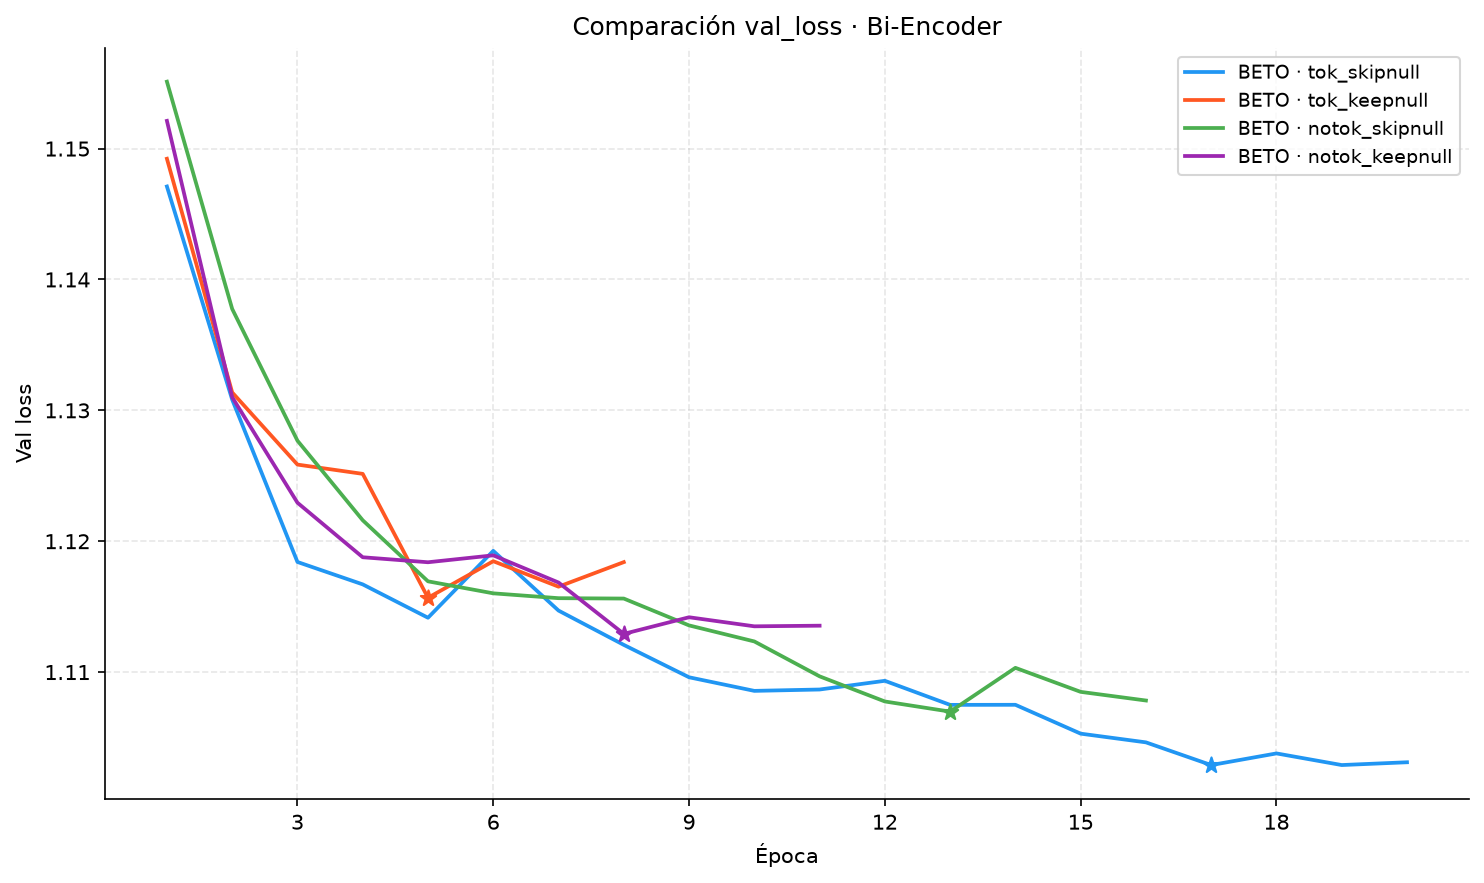
\includegraphics[width=0.90\textwidth]{Figuras/biencoder_serialization_comparison.png}
    \caption{Pérdida de validación por época para las cuatro variantes de serialización del Bi-Encoder BETO. Las estrellas indican el checkpoint de menor pérdida de cada corrida.}
    \label{fig:biencoder_serialization_comparison}
\end{figure}

La Figura~\ref{fig:biencoder_serialization_comparison} muestra además una diferencia en la dinámica de optimización. Las dos variantes que omiten nulos conservaron mejoras durante más épocas. La configuración \texttt{tok\_skipnull} alcanzó su mejor checkpoint en la época 17 y ejecutó 20 épocas; \texttt{notok\_skipnull} alcanzó su mínimo en la época 13 y ejecutó 16. En cambio, los mejores checkpoints de \texttt{tok\_keepnull} y \texttt{notok\_keepnull} ocurrieron en las épocas 5 y 8, y las corridas finalizaron por \textit{early stopping} en las épocas 8 y 11, respectivamente, sin recuperar una mejora sostenida de la pérdida de validación.

La omisión de valores nulos evita repetir información ausente que no discrimina entidades y permite que el modelo continúe refinando la representación con las observaciones disponibles. Los tokens estructurales, por su parte, conservan la delimitación entre bloques y pares clave-valor. Esta combinación permite al modelo identificar qué tipo de información representa cada fragmento sin sobrecargar la secuencia con ausencias. La ventaja en separación es moderada frente a \texttt{notok\_skipnull}, por lo que la conclusión debe interpretarse como una selección empírica dentro de este conjunto de datos y no como una regla universal.


% ==============================================================================
% 5.2 RECUPERACIÓN CON BI-ENCODER
% ==============================================================================
\section{Recuperación eficiente: Bi-Encoder}

Como referencia, se evaluaron sin ajuste fino BETO, RoBERTa-biomedical y paraphrase-multilingual sobre la variante \texttt{notok\_skipnull}. La Tabla~\ref{tab:zeroshot_resultados} muestra que ninguno de los modelos preentrenados produce una recuperación útil sin entrenamiento específico para el problema.

\begin{table}[htbp]
    \centering
    \small
    \caption{Promedios direccionales de los baselines zero-shot en test.}
    \label{tab:zeroshot_resultados}
    \begin{tabular}{lrrr}
        \hline
        Modelo & Recall@1 & MRR & $\Delta_{\mathrm{sep}}$ \\
        \hline
        BETO & 0.0051 & 0.0184 & 0.1583 \\
        RoBERTa-biomedical & 0.0045 & 0.0183 & 0.1651 \\
        paraphrase-multilingual & 0.0047 & 0.0248 & 0.1489 \\
        \hline
    \end{tabular}
\end{table}

Tras el entrenamiento contrastivo, el Bi-Encoder BETO con \texttt{tok\_skipnull} alcanza Recall@1 promedio de 0.9837, Recall@5 perfecto y MRR de 0.9998. La diferencia frente a los baselines confirma que la arquitectura preentrenada por sí sola no organiza los registros institucionales por identidad; el ajuste fino con pares cross-source es el componente que construye el espacio métrico útil para recuperación.


% ==============================================================================
% 5.3 HARD NEGATIVE MINING
% ==============================================================================
\section{Hard Negative Mining}

Con la variante canónica se recuperaron los 20 candidatos más similares por registro para construir los pares del Cross-Encoder. El procedimiento generó 8,513 pares positivos y 69,122 negativos difíciles en entrenamiento; 1,851 y 14,415 en validación; y 1,860 y 14,490 en test, respectivamente.

No se observaron positivos difíciles en las tres particiones: todos los pares positivos conocidos aparecieron en los primeros 20 candidatos. Este resultado confirma que el Bi-Encoder conserva la cobertura necesaria para la segunda etapa. Sin embargo, no demuestra cobertura sobre coincidencias ausentes del \textit{silver standard}; esa limitación se retoma en la discusión final.


% ==============================================================================
% 5.4 CLASIFICACIÓN FINA CON CROSS-ENCODER
% ==============================================================================
\section{Clasificación fina: Cross-Encoder}

El Cross-Encoder recibe los pares plausibles recuperados por el Bi-Encoder y decide si ambos registros pertenecen a la misma entidad. A diferencia de la primera etapa, procesa ambos textos conjuntamente y puede contrastar atributos específicos del par antes de emitir una puntuación. Se entrenó con BETO durante tres épocas sobre 8,513 positivos y 69,122 negativos difíciles, usando BCE ponderada con $\texttt{pos\_weight}=8$. La pérdida de validación descendió de 0.00233 en la primera época a $6.51\times10^{-5}$ en la tercera, que se seleccionó como checkpoint final.

La regla de decisión se ajustó de forma independiente al entrenamiento. Con el checkpoint final fijo, se puntuaron los 16,266 pares de validación y se evaluaron 51 umbrales uniformemente espaciados entre cero y uno. El máximo F1 de validación fue 1.0000 con $\tau=0.12$. Este umbral se congeló antes de evaluar el conjunto de prueba, por lo que las cifras de test no intervienen en su selección.

\begin{table}[htbp]
    \centering
    \small
    \caption{Evaluación del Cross-Encoder canónico en test con $\tau=0.12$.}
    \label{tab:cross_encoder_results}
    \begin{tabular}{l r}
        \hline
        Métrica & Valor \\
        \hline
        Pares evaluados & 16,350 \\
        F1 & 0.9997 \\
        Precisión & 1.0000 \\
        Recall & 0.9995 \\
        Exactitud & 0.9999 \\
        PR-AUC / ROC-AUC & 1.0000 / 1.0000 \\
        Verdaderos positivos / negativos & 1,859 / 14,490 \\
        Falsos positivos / negativos & 0 / 1 \\
        \hline
    \end{tabular}
\end{table}

La distribución de puntuaciones confirma la separación lograda en los pares candidatos: la media de los positivos fue 0.99943 (desviación estándar 0.02318), mientras que la de los negativos fue $2.90\times10^{-5}$ (desviación estándar $6.82\times10^{-5}$). Este resultado no implica que la tarea completa esté resuelta, pues mide solo los pares propuestos por la etapa de recuperación y las etiquetas disponibles constituyen un \textit{silver standard}.

La inspección del único falso negativo, correspondiente al caso PRADO APOLINAR, reveló una inconsistencia en el \textit{ground truth}: los registros atribuidos a una misma entidad contenían nombres y eventos incompatibles. El modelo asignó una puntuación de 0.0001 al par. Más que interpretar el caso como una prueba concluyente de exactitud, se considera evidencia de que el modelo puede apoyar la auditoría de etiquetas y priorizar casos para revisión humana. La calibración mediante \textit{temperature scaling} se ejecutó después de esta evaluación para analizar incertidumbre; no volvió a seleccionar ni modificó el umbral de decisión.


% ==============================================================================
% 5.5 VISUALIZACIÓN UMAP
% ==============================================================================
\section{Visualización del espacio métrico}

Para examinar cualitativamente la estructura aprendida por el Bi-Encoder, se proyectaron sus embeddings de 768 dimensiones a tres dimensiones mediante UMAP (\textit{Uniform Manifold Approximation and Projection})~\cite{mcinnes2018}. UMAP construye primero un grafo ponderado de vecindades en el espacio original y después optimiza una representación de baja dimensionalidad que preserva, en lo posible, esas relaciones locales. Esta técnica permite inspeccionar en una misma figura cómo se distribuyen registros de distintas fuentes y si las observaciones de una misma entidad ocupan vecindades comunes; no se utiliza como medida de desempeño ni como sustituto de la evaluación de recuperación.

La Figura~\ref{fig:umap_entidad_471} muestra una vista 3D de los registros pertenecientes a entidades observadas en más de una fuente. Cada punto corresponde a un registro y el color identifica su base de origen. Las anotaciones destacan los tres registros de la entidad 471, correspondientes a JUAN SANCHEZ LAGUNES, provenientes de Económico, Comorbilidad y Trabajo Social. Los tres puntos se encuentran en la misma vecindad local a pesar de las variaciones en el orden del nombre entre fuentes, lo que ilustra el comportamiento que se busca inducir mediante el entrenamiento contrastivo.

\begin{figure}[htbp]
    \centering
    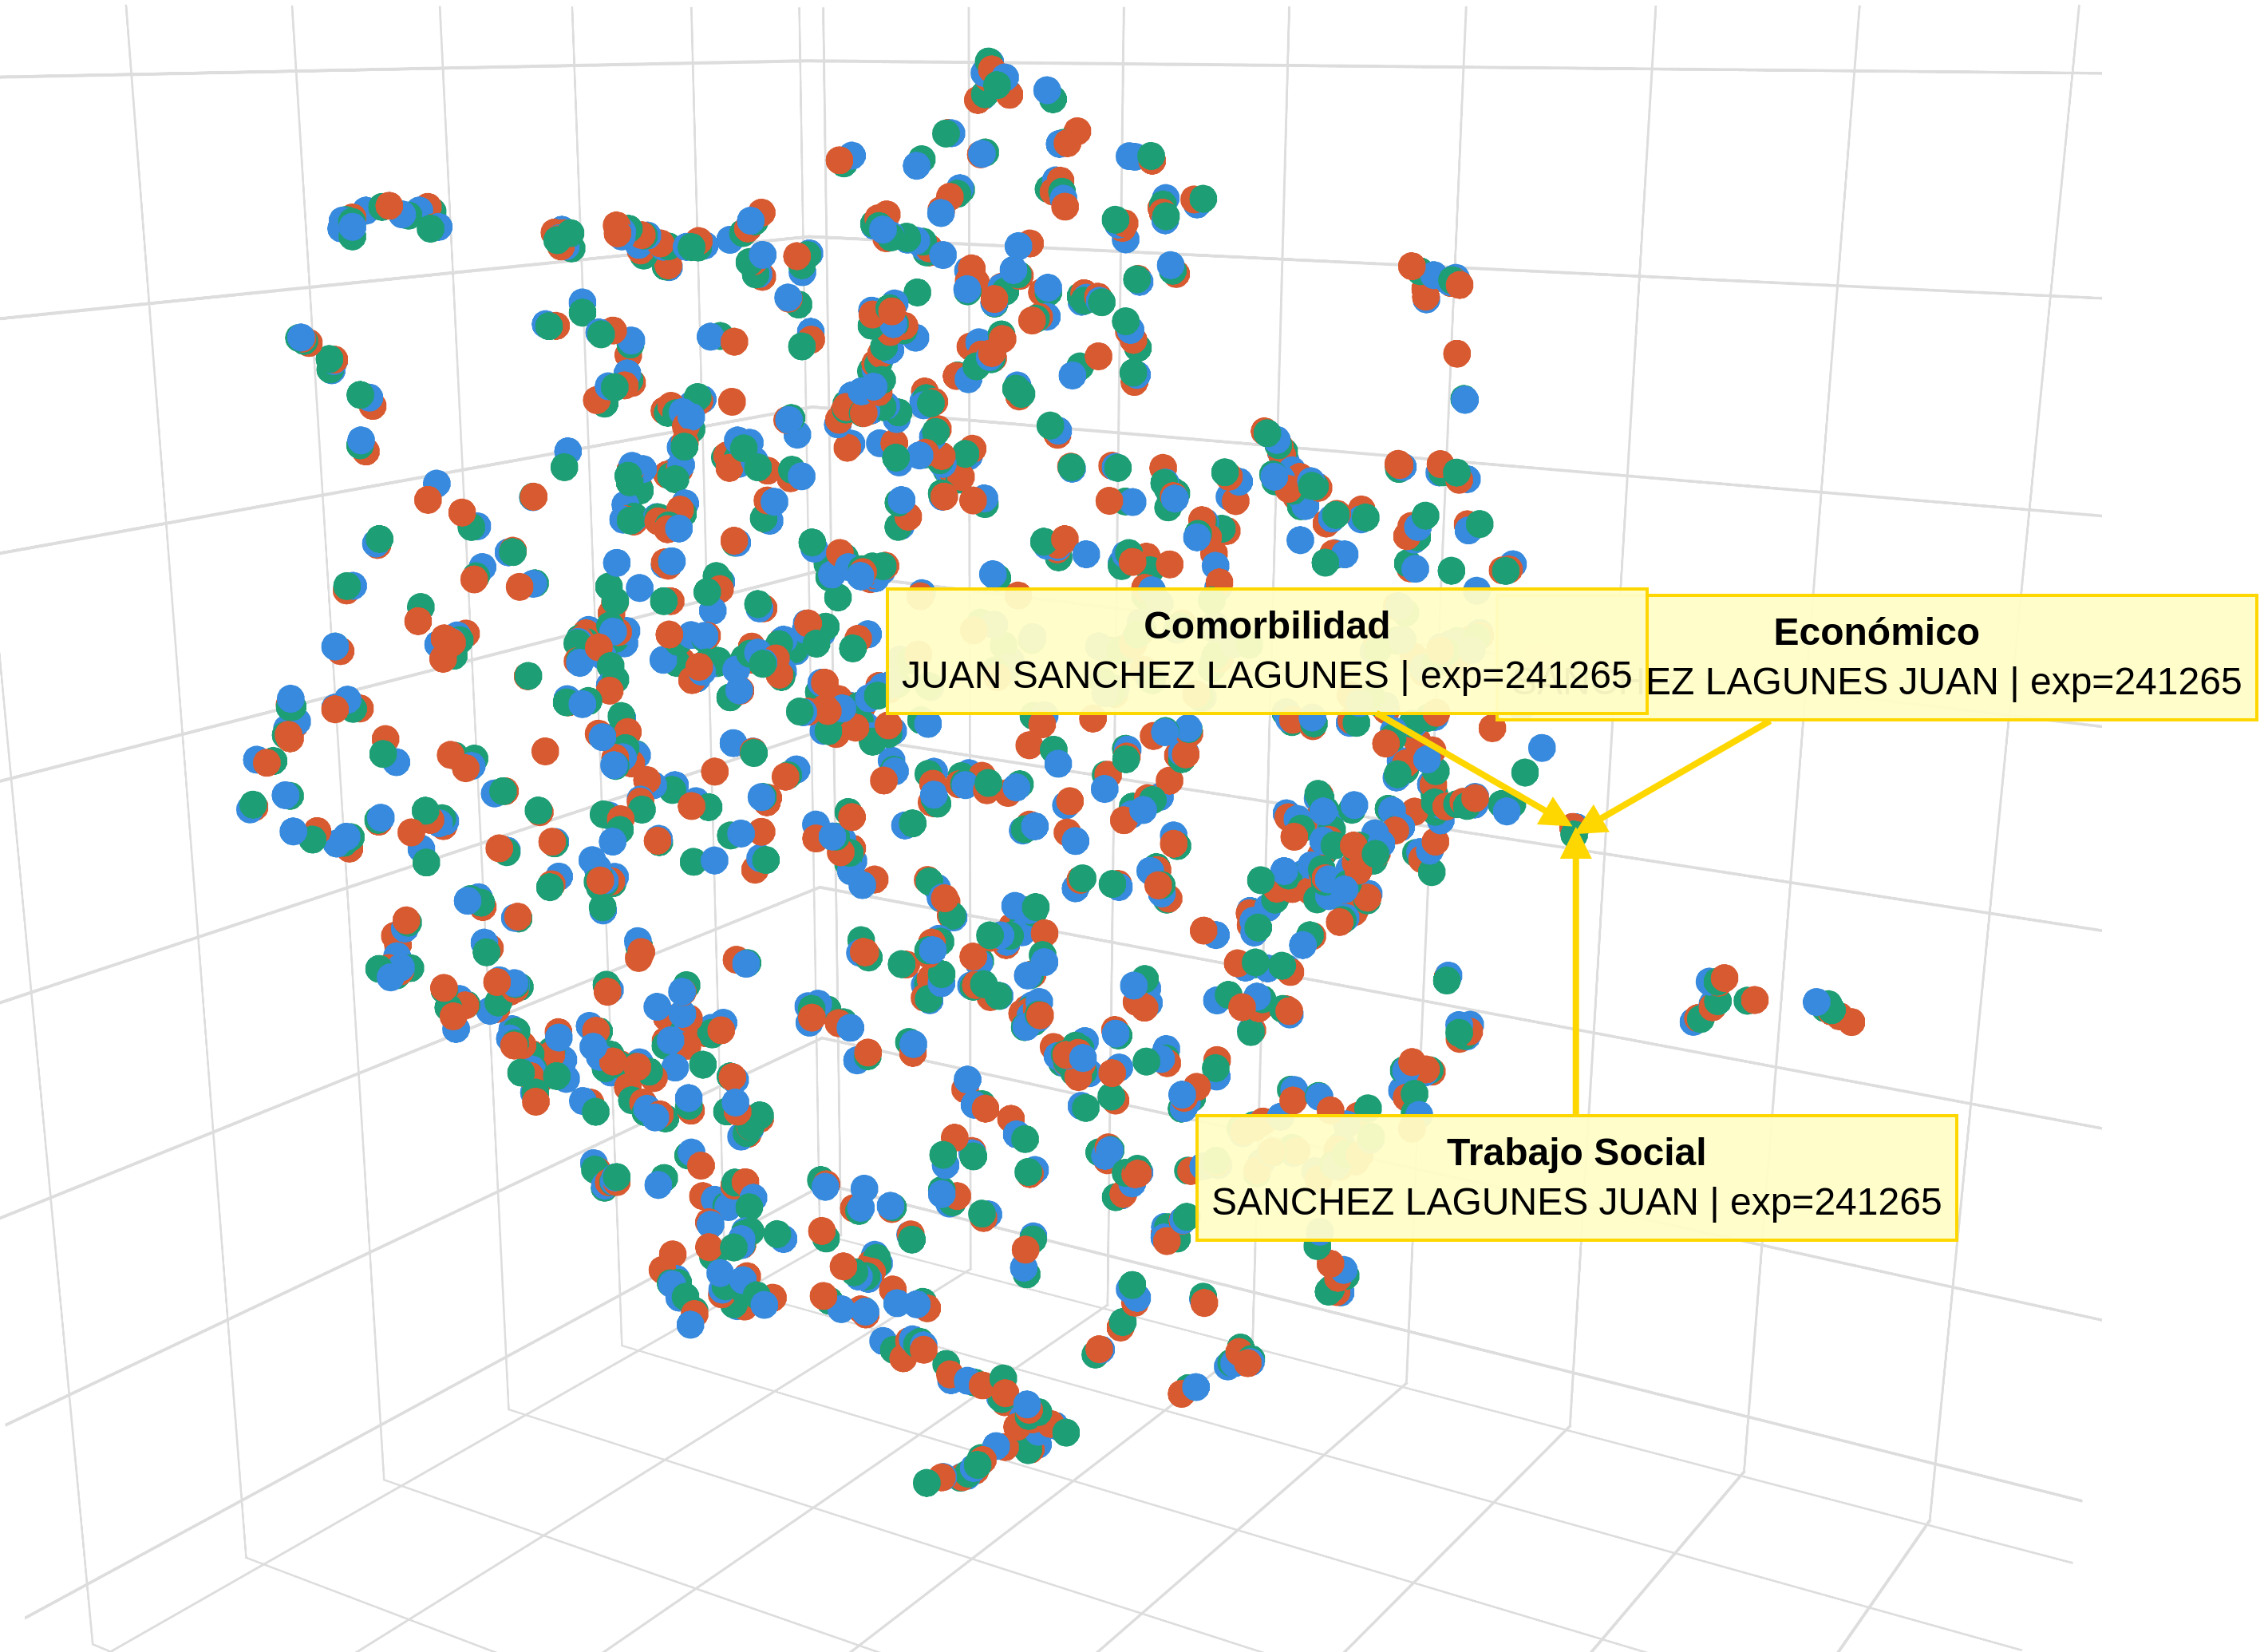
\includegraphics[width=\textwidth]{Figuras/umap_entidad_471_poster.png}
    \caption{Proyección UMAP tridimensional del espacio métrico aprendido por el Bi-Encoder. Cada punto representa un registro de una entidad presente en más de una fuente y el color identifica la base de origen. Las anotaciones resaltan los tres registros de la entidad 471, que quedan ubicados en una misma vecindad local.}
    \label{fig:umap_entidad_471}
\end{figure}

La proximidad visual de esos puntos es consistente con las métricas de recuperación y separación reportadas anteriormente, pero su interpretación debe mantenerse acotada. UMAP privilegia la preservación de estructura local y puede distorsionar distancias globales; por tanto, la figura sirve para comunicar y diagnosticar el espacio aprendido, no para demostrar por sí sola la cobertura de coincidencias no observadas ni la calidad del sistema completo.


% ==============================================================================
% 5.6 CALIBRACIÓN E INCERTIDUMBRE
% ==============================================================================
\section{Calibración e incertidumbre}

La calibración mediante \textit{temperature scaling} se ejecutó después de fijar el umbral y no modificó la regla de decisión. Sobre validación, el ajuste produjo $T=0.065256$, con ECE de $3.7\times10^{-5}$ antes de calibrar y 0 después. La validación perfectamente separable hizo que la transformación llevara las probabilidades calibradas a valores extremos; en test, la entropía calibrada media fue prácticamente nula.

Por esta razón, el diagnóstico de ambigüedad se realizó con la entropía de la puntuación cruda. Nueve de los 16,350 pares de test alcanzaron $H(p)\geq0.01$ bits; ninguno superó 0.1 bits. El Parquet de incertidumbre conserva, por par, la puntuación cruda, la probabilidad calibrada, ambas entropías y el margen respecto de $\tau=0.12$. El caso PRADO ilustra el límite de esta lectura: una predicción muy confiada puede discrepar de una etiqueta que posteriormente requiere revisión. La incertidumbre cuantificada se limita a los pares que llegan al Cross-Encoder; no incorpora posibles coincidencias que la etapa de recuperación no haya propuesto.


% ==============================================================================
% 5.7 DISCUSIÓN INTEGRADORA
% ==============================================================================
\section{Discusión integradora}

El sistema \textit{Retrieve \& Re-rank} logra una recuperación de alta cobertura y una clasificación casi perfecta respecto del \textit{silver standard} disponible. La comparación entre variantes identifica a \texttt{tok\_skipnull} como la mejor configuración dentro del experimento, aunque la ventaja en separación frente a \texttt{notok\_skipnull} es reducida. Esta conclusión se sostiene en pérdida de validación y $\Delta_{\mathrm{sep}}$, pues las métricas de ranking se saturan en el conjunto de prueba.

El resultado no equivale a una validación clínica ni a una garantía de que se recuperen todas las coincidencias reales. Las etiquetas fueron construidas mediante un proceso de consolidación y revisión, por lo que pueden conservar errores o coincidencias no observadas. En consecuencia, el sistema debe entenderse como un apoyo a la integración de registros y a la priorización de revisión humana, no como un sustituto autónomo de validación institucional.
